\begin{figure}[t]
  \hspace{0.125\textwidth}%
  \begin{subfigure}[b]{\textwidth}
    \tikzstyle{legend-point}=[circle, inner sep=2pt]
    \definecolor{GraphBlue}{HTML}{6c8abd}
    \definecolor{GraphGreen}{HTML}{73b584}
    \definecolor{GraphRed}{HTML}{d07175}

    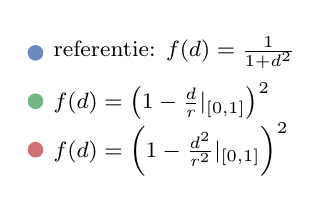
\begin{tikzpicture}
      \node (legend:basic) at (0.1\textwidth,0) [legend-point, fill={GraphBlue}, label=right:{\footnotesize referentie: $f(d) = \frac{1}{1 + d^2}$} ] {};
      \node (legend:d) at (0.1\textwidth, -17.5pt) [legend-point, fill={GraphGreen}, label=right:{\footnotesize $f(d) = \left( 1 - \frac{d}{\mathit{r}}|_{[0,1]} \right)^2$} ] {};
      \node (legend:d2) at (0.1\textwidth, -35pt) [legend-point, fill={GraphRed}, label=right:{\footnotesize $f(d) = \left( 1 -  \frac{d^2}{\mathit{r}^2}|_{[0,1]} \right)^2$} ] {};
    \end{tikzpicture}
  \end{subfigure}\hfill\\
  \begin{adjustbox}{minipage=\textwidth, scale=1.0}
    \centering
    \begin{subfigure}[b]{0.8\textwidth}
      \centering
      \def\svgwidth{\textwidth}
      \input{./img/raw/th-light-att/attenuation_func.pdf_tex}
    \end{subfigure}
  \end{adjustbox} %
  \caption{Afstandsdempingscurves voor eindige omnipuntlichtbronnen.}
  \label{fig:pl-distance-attenuation}
\end{figure}

